\documentclass{beamer}
\usetheme{Amsterdam}

\usepackage[utf8]{inputenc}
\usepackage[T1]{fontenc}
\usepackage{cmap}
\usepackage{listings}
\lstset{language=C}

\title{\textbf{RapidFit}\newline~A beginners Guide, Talk 1 of ?}
\author{\textbf{Robert Currie}, Edinburgh University\newline\hspace{.5cm} \textcolor{white}{\textbf{\insertframenumber \vspace{-.33cm}/ \vspace{-.33cm}\inserttotalframenumber}}}
\date{}

\usepackage{color}
\definecolor{gray}{rgb}{0.4,0.4,0.4}
\definecolor{darkblue}{rgb}{0.0,0.0,0.6}
\definecolor{cyan}{rgb}{0.0,0.6,0.6}

\begin{document}

\lstset{
  basicstyle=\ttfamily,
  columns=fullflexible,
  showstringspaces=false,
  commentstyle=\color{gray}\upshape
}

\lstdefinelanguage{XML}
{
  morestring=[b]",
  morestring=[s]{>}{<},
  morecomment=[s]{<?}{?>},
  stringstyle=\color{black},
  identifierstyle=\color{darkblue},
  keywordstyle=\color{cyan},
  morekeywords={xmlns,version,type}% list your attributes here
}

\begin{frame}
\titlepage
\end{frame}

\section{Intro}

\begin{frame}
 \frametitle{Introduction}
 \begin{itemize}
  \item How To Setup RapidFit. \textbf{(Properly!)}.\newline
  \item What is a PDF in RapidFit?\newline
  \item My First PDF \& XML\newline
  \item My First Projection\newline
  \item My First $\Delta$LL Scan\newline
  \item My First Toy Study\newline
  \item Analysing My Output(s)\newline
  \end{itemize}
\end{frame}

\begin{frame}
\frametitle{Next Week and Future Talks...}
\begin{itemize}
\item Expanding Upon DataSet(s)
\item More on $\Delta$LL Scans
\item My First $\Delta$LL Contour
\item More on Projections
\item More on Toy Studies
\item More on XML Options
\item More Runtime Arguments
\item Running on ECDF/The Grid
\item Complex studies with RapidFit
\item Commonly used RapidFit C++ objects
\item Some features of the utils codebase
\item ...Anything else? What are people most eager to have a tutorial on?
\end{itemize}
\end{frame}

\begin{frame}
\frametitle{Introduction}
All of the code will be available soon. (my work on $J/\psi~\phi$ willing)\newline

All of the XML I present will be made available in svn HEAD\newline(They are not there at this time, apologies)\newline

The more feedback I get the more I can improve future talks/documentation.

\end{frame}

\section{Setup}

\begin{frame}
 \frametitle{What do I need to Get RapidFit Setup?}
 \begin{itemize}
  \item CERN computing account\newline(preferably with lxplus/AFS privileges)\newline
  \item Access to RapidFit repository\newline(speak to Dean Lambert \@ CERN)\newline
  \item UNIX skills (ssh, make, gcc, etc)\newline
  (We have NO plans to support windows. EVER!)\newline
  \item This Tutorial\newline
  \end{itemize}
  (alternatively speak to myself and I will advise you on what to do)
\end{frame}

\begin{frame}
\frametitle{What Does RapidFit Need?}
\begin{itemize}
 \item ROOT\newline
 Almost everything you do in PPE relies on ROOT.\newline
 It's a love-hate relationship, try to get past the fact it's ugly.\newline
 \item bash\newline
 RapidFit and a lot solutions I can provide are bash based.\newline
 \item (Otional) GSL libraries\newline
 This is required for few special analyses, but is available for everyone to use.\newline
 \item UNIX\newline
 We rely on common POSIX and STL over ROOT solutions.\newline
 \item Future dependencies/developments include: CUDA / OpenCL\newline
 Ask Dianne
\end{itemize}
\end{frame}

\begin{frame}
\frametitle{How to Setup RapidFit}
 \begin{itemize}
  \item Firstly Get the RapidFit source code:\newline
  \tiny svn co svn+ssh://cern-username@svn.cern.ch/reps/lhcbedinburgh/Code/Fitting/RapidFit/trunk\normalsize\newline
  \item Configure ROOT:
  \begin{itemize}
   \item on lxplus: SetupProject ganga
   \item compile it yourself with '--all' and\newline 'source /some/path/thisroot.sh'
   \item install from your distro's Repo i.e. Ubuntu (ask Google)
   \item compile using homebrew and XCode on OSX (ask Google)
   \item We rely on many ROOT 'optional' tools. When in doubt:\newline Don't build yourself!\newline
  \end{itemize}
  \item Optional make sure gsl-config is in your \$PATH\newline
  \item Build RapidFit with 'make' or 'make all'
 \end{itemize}
\end{frame}

\begin{frame}
\frametitle{Building RapidFit}
\begin{itemize}
 \item RapidFit uses GNU make.\newline
 This simply generates a lot of gcc commands to build source.\newline
 This is configured by the 'Makefile' in the top of the trunk.\newline
 \item The options to make you should know are:
 \small
 \begin{itemize}
  \item make or 'make all'\newline
  This builds everything
  \item make utils\newline
  This builds the tools in the utils folder
  \item make bin/fitting\newline
  This builds RapidFit
  \item make gsl\newline
  This builds RapidFit with optional GSL addons.
  \item make clean\newline
  Clear the old build files after the code has changed\newline~Use after 'svn up'
 \end{itemize}
\end{itemize}
\end{frame}

\begin{frame}
\frametitle{Why use Compiled Code?}

There are several extremely good reasons as to why we use compiled code:

\begin{itemize}
 \item It's faster
 \item The compiler knows better C++ than me!
 \item The compiler knows better C++ than you!
 \item It's really, really fast
 \item It forces you to think about what you're doing
 \item Stops problems due to really bad code that can be in CINT
\end{itemize}

\textbf{ALWAYS}: rebuild after changing your code.\newline

\textbf{BEFORE}: you claim you've found a bug can you repeat it after a make clean?


\end{frame}


\section{XML\&PDF}

\begin{frame}[fragile]
\frametitle{XML \&~PDF}
In order to run your fit you need to have an XML to configure RapidFit.\newline

The XML consists of:\small
\begin{itemize}
 \item ParameterSet\newline
 What am I trying to measure?\newline
 \item ToFit(s)\newline
 What am I trying to use to make a measurement?\newline
 \item FitFunction\newline
 How am I defining how well my ParameterSet matches the ToFit(s)\newline
 \item Minimiser\newline
 What I am using to calculate the best ParameterSet for my ToFit(s)
\end{itemize}


\end{frame}

\begin{frame}[fragile]
And a simple XML, one can fit on a single overhead!
\lstset{
  language=XML,
  morekeywords={encoding,
  xs:schema,xs:element,xs:complexType,xs:sequence,xs:attribute}
}\tiny
\begin{lstlisting}[tabsize=8]
<RapidFit>
<ParameterSet>
<PhysicsParameter>
<Name>sigma</Name>
<Minimum>0.</Minimum>
<Maximum>5.</Maximum>
</PhysicsParameter>
</ParameterSet>
<Minimiser>Minuit</Minimiser>
<FitFunction>NegativeLogLikelihood</FitFunction>
<ToFit>
<PDF>
<Name>SimpleGauss</Name>
</PDF>
<DataSet>
<Source>Foam</Source>
<NumberEvents>1000</NumberEvents>
<PhaseSpaceBoundary>
<Observable>
<Name>x</Name>
<Minimum>-10.</Minimum>
<Maximum>10.</Maximum>
</Observable>
</PhaseSpaceBoundary>
</DataSet>
</ToFit>
</RapidFit>
\end{lstlisting}

\end{frame}

\begin{frame}
\frametitle{A simple PDF}
OK so I have a simple fit in mind:\newline\newline

1: PhysicsParameter: sigma\newline
1: Observable: x\newline
1: PDF: 'SimpleGauss'\newline
1: DataSet: Foam 1,000 events\newline
\newline

How do I construct SimpleGauss to allow me to do this?

\end{frame}

\begin{frame}
\frametitle{Constructing SimpleGauss}

XML requirements:\newline\newline

SimpleGauss has to be constructed to tell RapidFit what Observables it expects to be provided. (x)\newline
This is done by populating: SimpleGauss::allObservables;\newline\newline


It also has to tell RapidFit what PhysicsParameters it wants to measure.(sigma).\newline
This is done by populating: SimpleGauss::allParameters;\newline\newline

\end{frame}

\begin{frame}
\frametitle{Constructing SimpleGauss}
C++ Requirements:\newline

SimpleGauss must 'advertise' itself to RapidFit as a PDF:\newline
use:\newline  PDF\_CREATOR( SimpleGauss );\newline

SimpleGauss must provide a method to Evaluate the Probability of finding a DataPoint:\newline
SimpleGauss::Evaluate( DataPoint* );\newline

SimpleGauss should (not must) provide a method to Normalise the Probability of finding a DataPoint in a whole PhaseSpace.\newline\newline
SimpleGauss::Normalise( PhaseSpaceBoundary* ); or
SimpleGauss::Normalise( DataPoint*, PhaseSpaceBoundary* )


\end{frame}

\begin{frame}[fragile]
\frametitle{Constructing SimpleGauss PDF}
\lstset{language=C++,
basicstyle=\ttfamily,
keywordstyle=\color{blue}\ttfamily,
stringstyle=\color{red}\ttfamily,
commentstyle=\color{green}\ttfamily,
morecomment=[l][\color{magenta}]{\#}
}\tiny
\begin{lstlisting}[tabsize=8]
#include "SimpleGauss.h"
#include <string>
#include <vector>
#include <cmath>
using namespace::std;
PDF_CREATOR( SimpleGauss );
SimpleGauss::SimpleGauss( PDFConfigurator* config ) :
  xName( "x" ), sigmaName( "sigma" )
{  this->MakePrototypes();  }
void SimpleGauss::MakePrototypes()
{
  allObservables.push_back( string(xName) );
  allParameters = ParameterSet( vector<string>( 1, string(sigmaName)) );
}
SimpleGauss::~SimpleGauss() {}
double SimpleGauss::Evaluate( DataPoint* input )
{
  double sigmaVal = allParameters.GetPhysicsParameter( sigmaName )->GetValue();
  double xVal = input->GetObservable( xName )->GetValue();
  double numerator = exp(-(xVal*xVal)/(2.*sigmaVal*sigmaVal));
  return numerator;
}
double SimpleGauss::Normalisation( PhaseSpaceBoundary* range )
{
  double sigmaVal = allParameters.GetPhysicsParameter( sigmaName )->GetValue();
  double denominator =(sigmaVal*sqrt(2.*Mathematics::Pi()));
  return denominator;
}
\end{lstlisting}

\end{frame}

\begin{frame}
 \frametitle{Running the Fit}
 In order to run RapidFit you need to know the options to pass to it.\newline\newline
 RapidFit as a binary when you have built the code is:\newline './bin/fitting'\newline\newline
 A standard fit of one XML is run by using:\newline
 \begin{center}
 'fitting -f someXML.xml'\newline
 \end{center}

 Some basic help and information exists:\newline
 'fitting --help' and 'fitting --about'\newline\newline
 More about the various Runtime options next week.
\end{frame}

\begin{frame}[fragile]
\frametitle{Aside- Where is My Data coming from?}
In this example, and as with all Toy Studies and simple tests of the PDF the Data is generated using the PDF itself.\newline\newline
This is because I have used:
\lstset{
  language=XML,
  morekeywords={encoding,
  xs:schema,xs:element,xs:complexType,xs:sequence,xs:attribute}
}\tiny
\begin{lstlisting}[tabsize=8]
<DataSet>
<Source>Foam</Source>
...
</DataSet>
\end{lstlisting}

\normalsize When this source of Data is used the ParameterSet in the XML is taken to be the truth or CV to be used in constructing the DataSet.\newline\newline
The only function in the PDF used for generating the DataSet is PDF::Evaluate( DataPoint* );\newline

More on this when it becomes important!
\end{frame}

\begin{frame}
\frametitle{How do I process Output?}
I have written a nice tool which does 90\%+ of what you want a tool to do in post-processing from the RapidFit Results.\newline

It is called 'RapidPlot'. You can pass it the output from toys, $\Delta$LL scans and contours as well as the results from FC analyses.\newline

The tool makes use of a highly modular code-base trying best to follow the 'rule of 7' (7 functions per class each with 7 lines each doing a specific job)\newline

Plots are almost publication ready (you may need to make tweaks for referee's but they're almost good enough to publish out of the box).
\end{frame}


\section{Projections}

\begin{frame}[fragile]
\frametitle{My First Projection}
Projections allow us to get a handle on the question of:\newline
``How well does my Fit Describe this Observable?''\newline\newline

In order to run a projection in RapidFit you need to add a new XML segment to the file:
\lstset{
  language=XML,
  morekeywords={encoding,
  xs:schema,xs:element,xs:complexType,xs:sequence,xs:attribute}
}\tiny
\begin{lstlisting}[tabsize=8]
<Output>
<Projection>x</Projection>
</Output>
\end{lstlisting}
\normalsize~This tells RapidFit to project 'x' for all ToFit segments in my XML.\newline\newline
Projections allow you to determine how well you describe the distribution of a given Observable.\newline\newline
You can alternately use:
\lstset{
  language=XML,
  morekeywords={encoding,
  xs:schema,xs:element,xs:complexType,xs:sequence,xs:attribute}
}\tiny
\begin{lstlisting}[tabsize=8]
<Output>
<ComponentProjection>x</ComponentProjection>
</Output>
\end{lstlisting}

\small~(I will give more examples on this next week I'm covering enough for now.)

\end{frame}

\begin{frame}
\frametitle{My First Projection - Output}
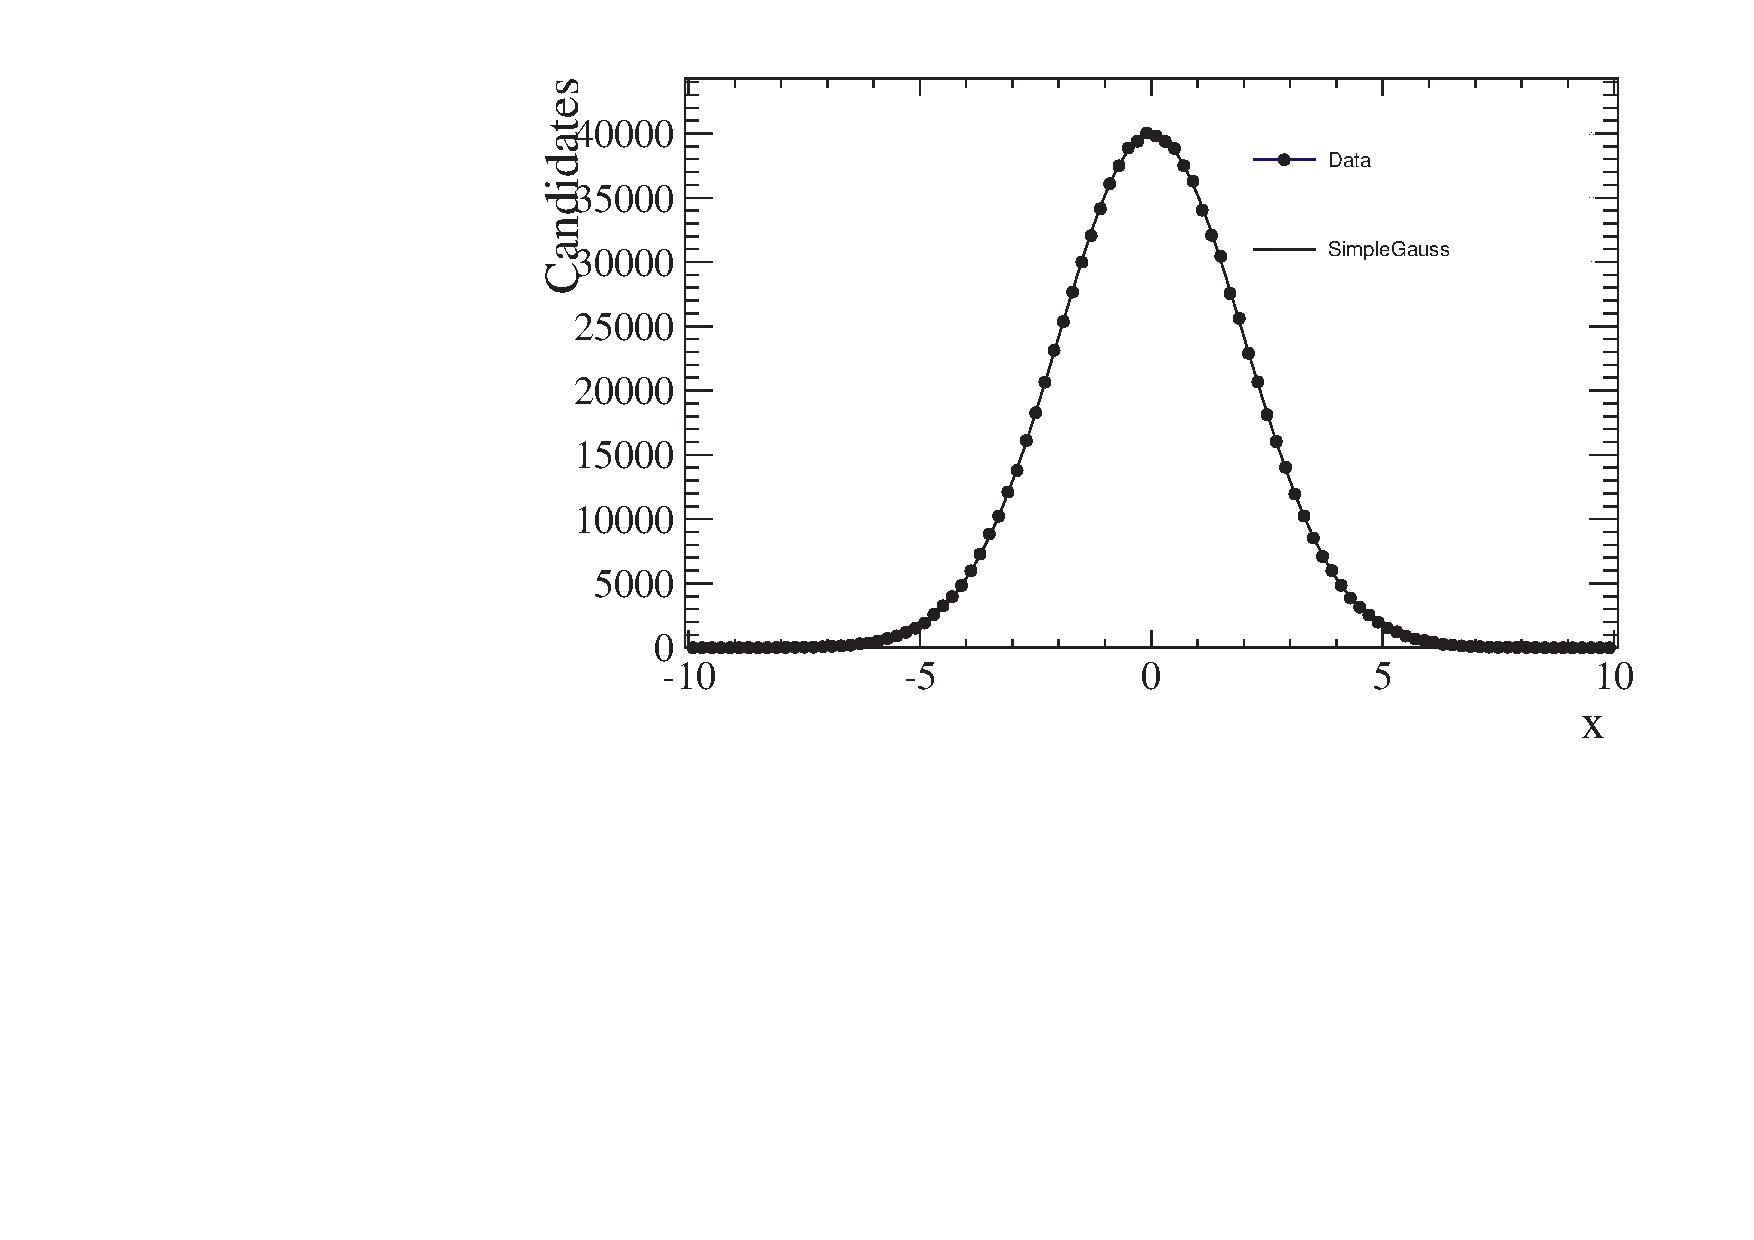
\includegraphics[width=\textwidth]{./Overlay_x_All_Data.pdf}
\end{frame}

\section{$\Delta$LLScan}
\begin{frame}[fragile]
\frametitle{My First $\Delta$LL Scan}

Running $\Delta$LL Scan(s) allow you to determine:\newline
``How well behaved is a given parameter in my fits?''\newline\newline

In order to perform a scan you need to add another section of XML to your XML file.
\lstset{
  language=XML,
  morekeywords={encoding,
  xs:schema,xs:element,xs:complexType,xs:sequence,xs:attribute}
}\tiny
\begin{lstlisting}[tabsize=8]
<Output>
<Scan>
<Name>sigma</Name>
<Sigma>3</Sigma>
<Points>100</Points>
</Scan>
</Output>
\end{lstlisting}
\normalsize
This code is NOT run by default when you run a fit, you need to request it to be run with '--doLLscan' when you launch RapidFit.

\end{frame}

\begin{frame}
\frametitle{My First $\Delta$LL Scan Output}
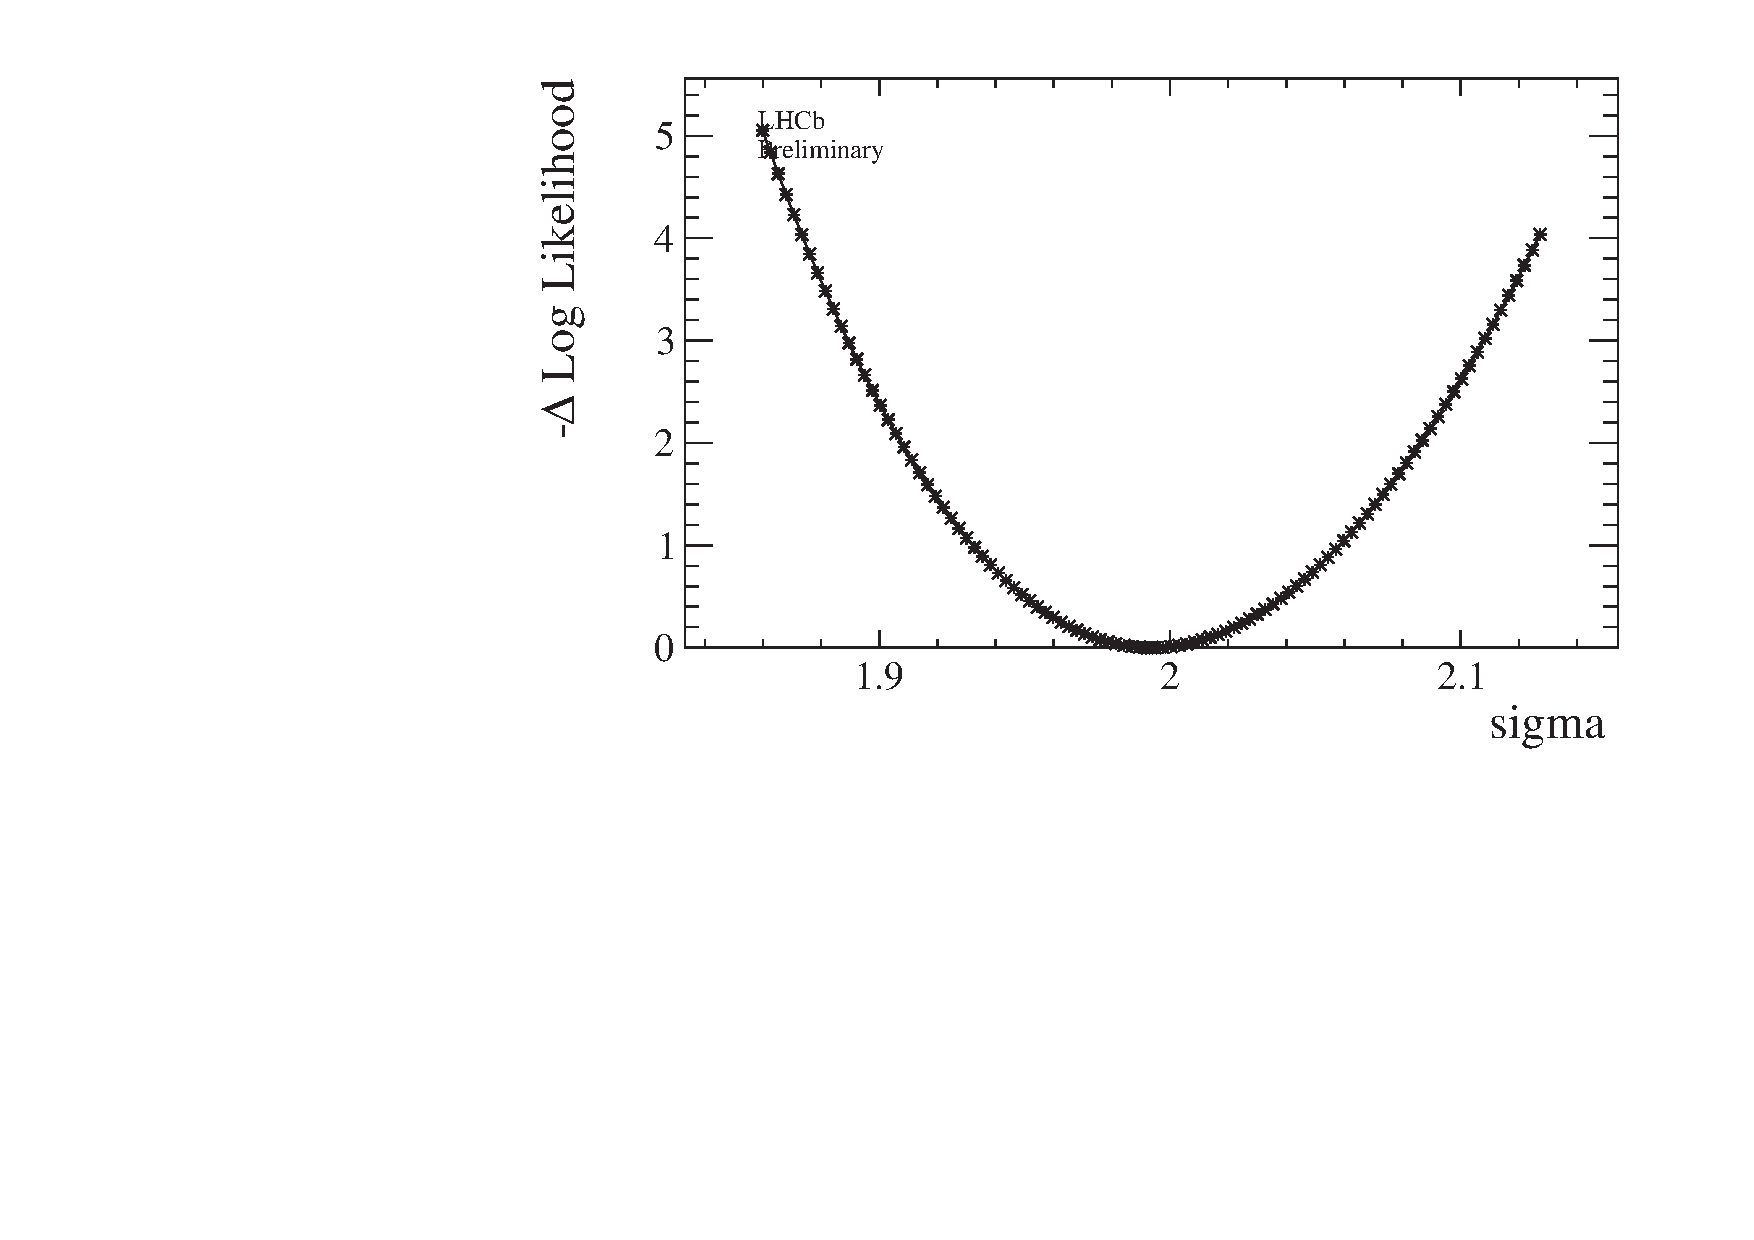
\includegraphics[width=\textwidth]{./RapidLL_sigma_conf.pdf}
\end{frame}

\section{Toy Studies}

\begin{frame}[fragile]
\frametitle{My First Toy Study}

Toy Studies allow you to address the question:\newline
``How Reproducible is my Result?''\newline\newline

To do this you need to repeat your fit with many toy Datasets.\newline

You can instruct RapidFit to do this in 2 ways:
XML:
\lstset{
  language=XML,
  morekeywords={encoding,
  xs:schema,xs:element,xs:complexType,xs:sequence,xs:attribute}
}
\begin{lstlisting}[tabsize=8]
<Repeats>100</Repeats>
\end{lstlisting}
or:\newline
pass '-repeats 100'\newline

to repeat 100 toys.

You generally want between 1,000 toys and 100,000 toys depending on how accurate you want to be about your statements.

\end{frame}

\begin{frame}
\frametitle{My First Toy Study Output (1k studies) }\begin{center}
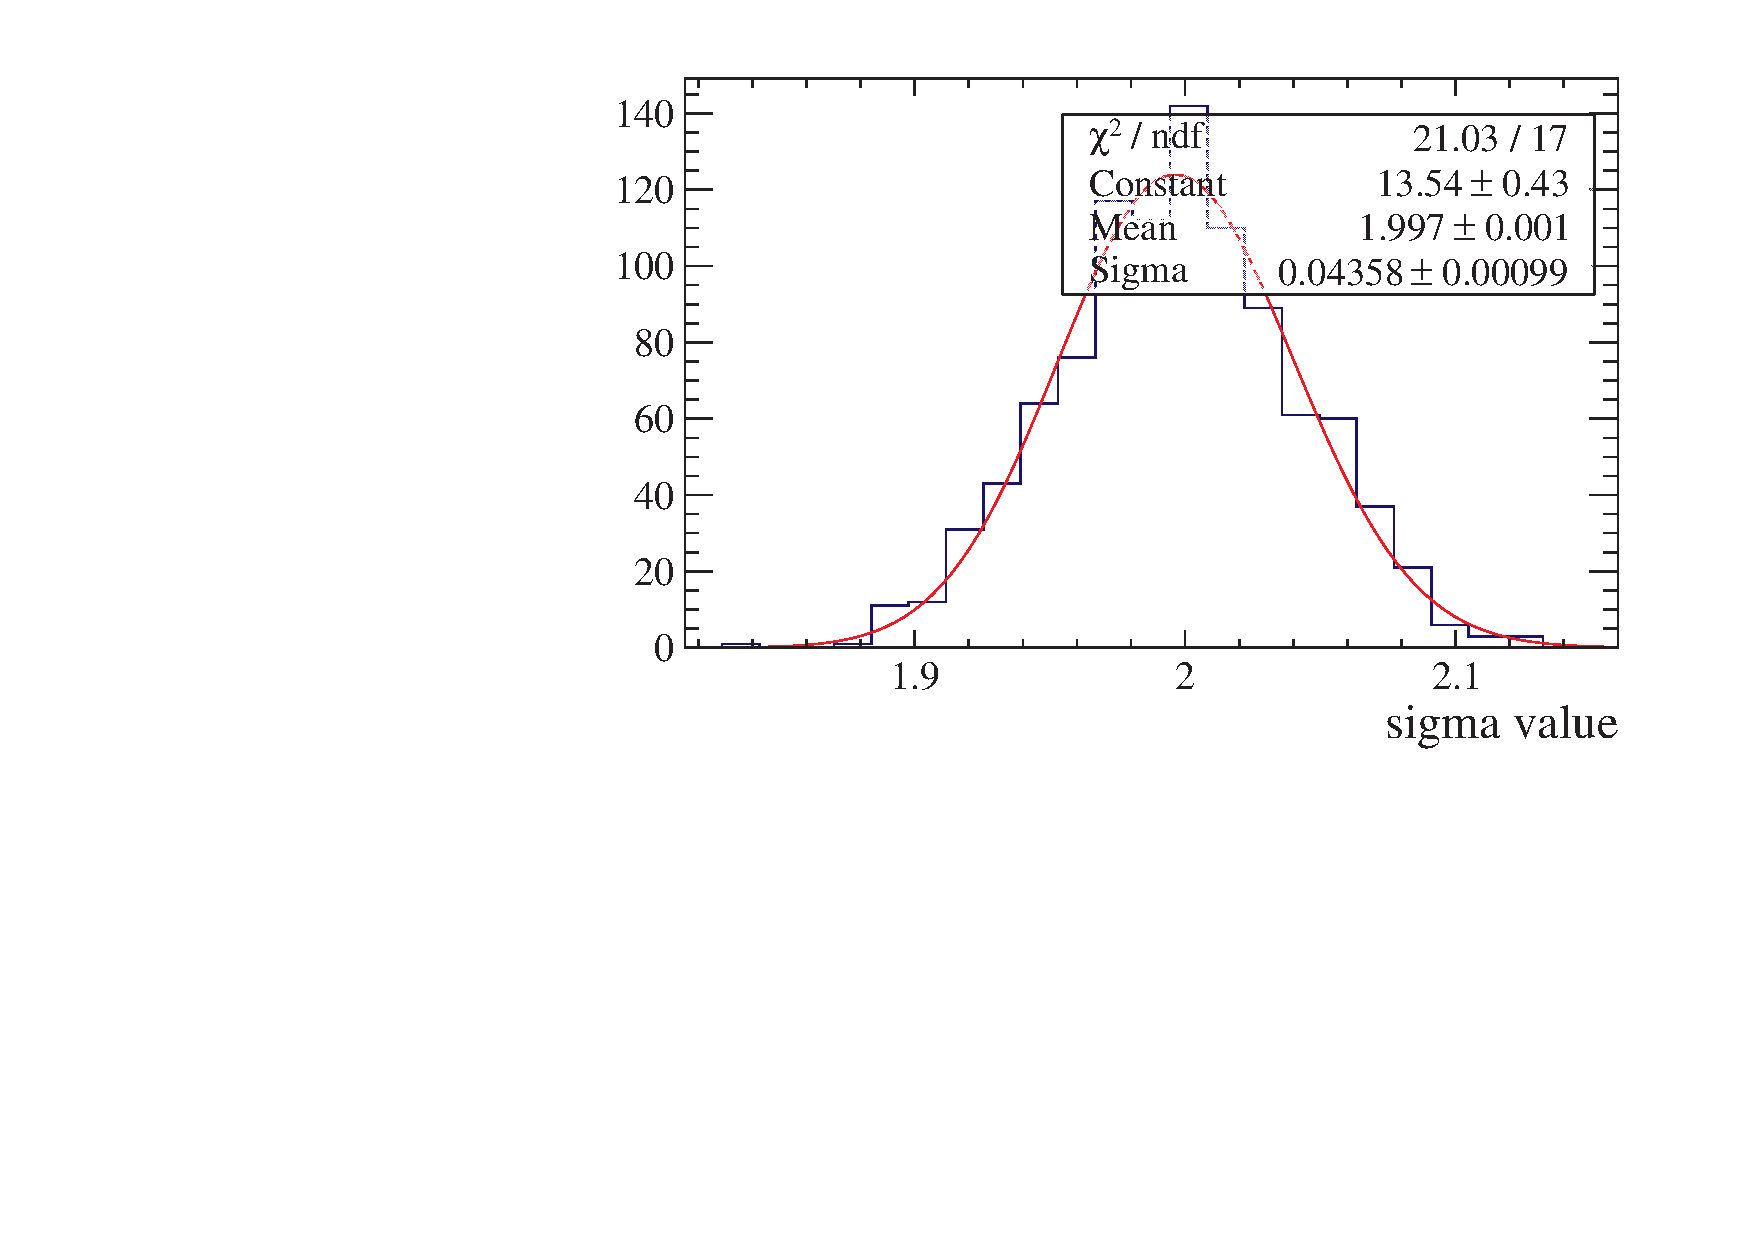
\includegraphics[width=0.5\textwidth]{./Output-1k/sigma_value_c_thru.pdf}
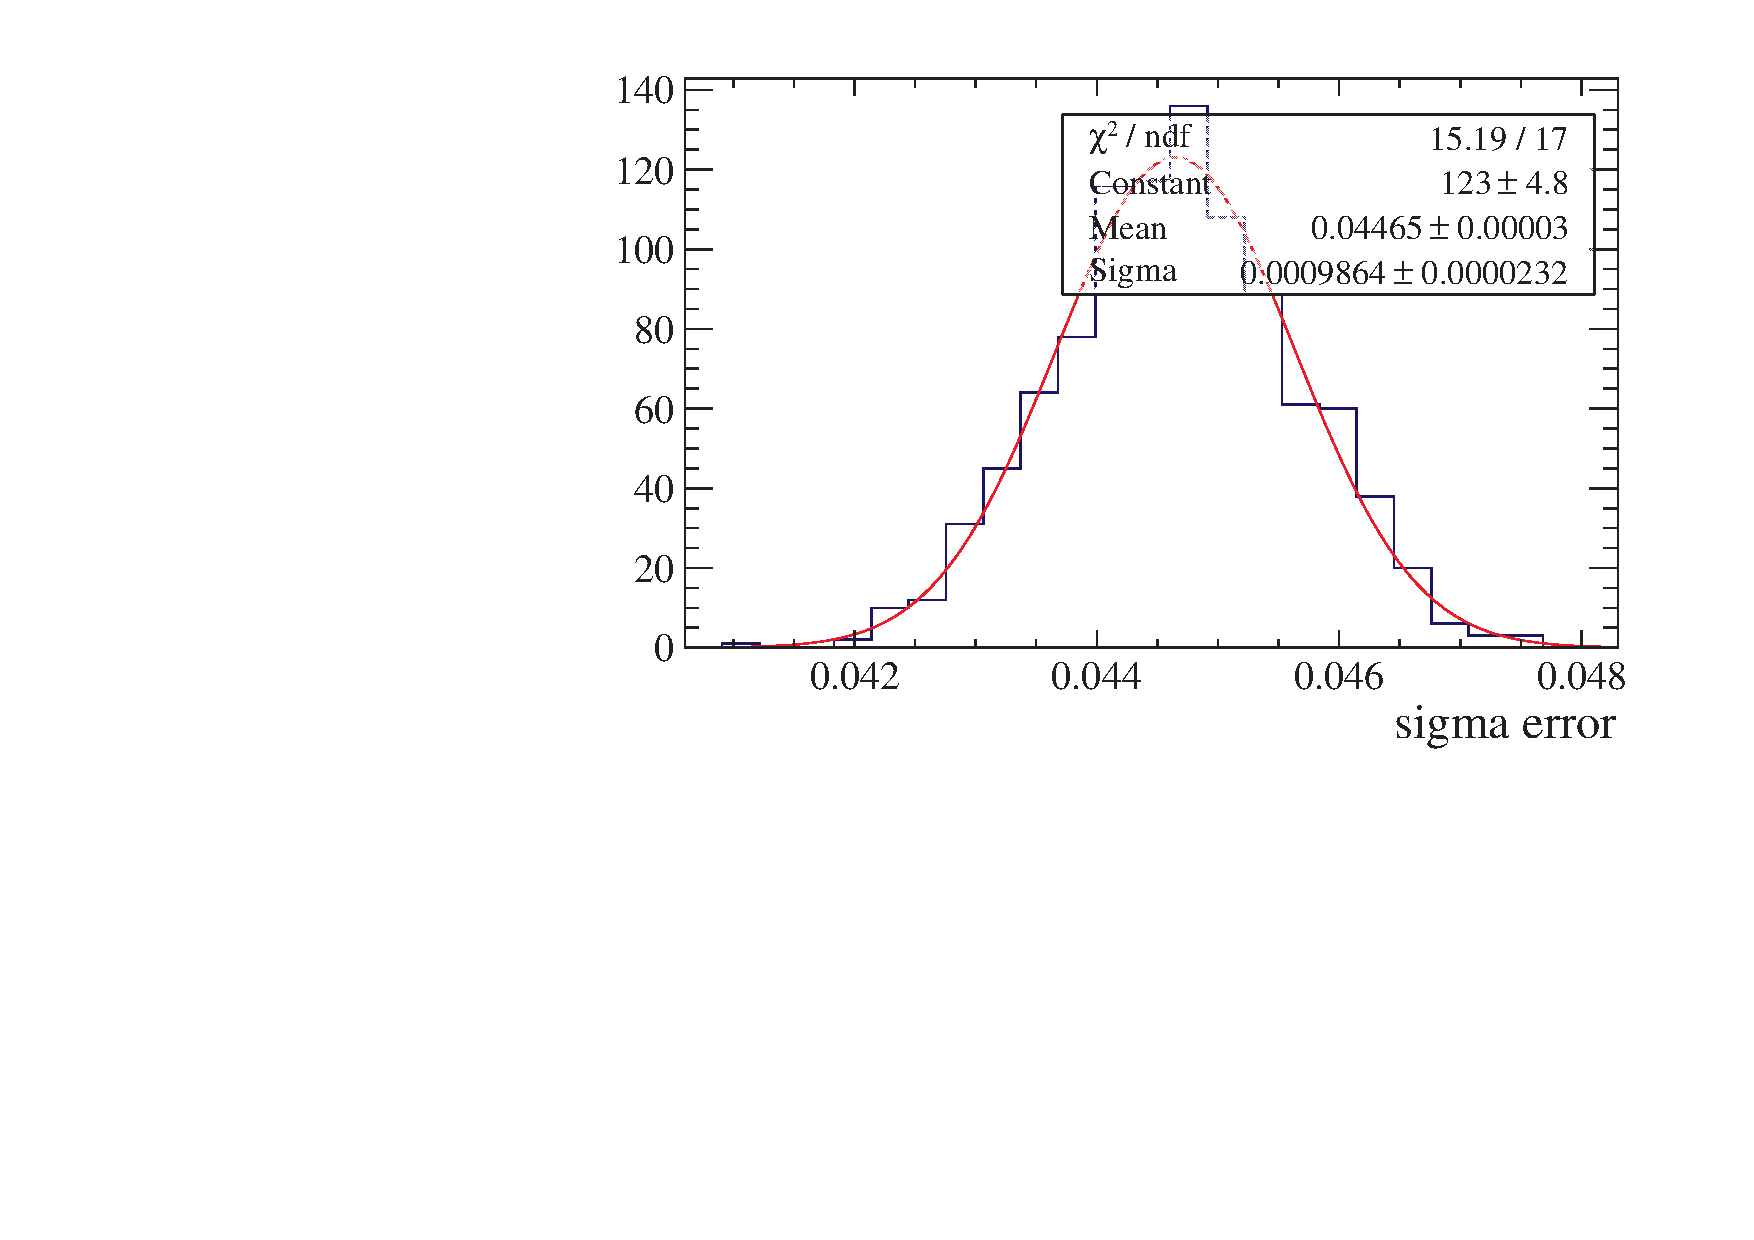
\includegraphics[width=0.5\textwidth]{./Output-1k/sigma_error_c_thru.pdf}\newline
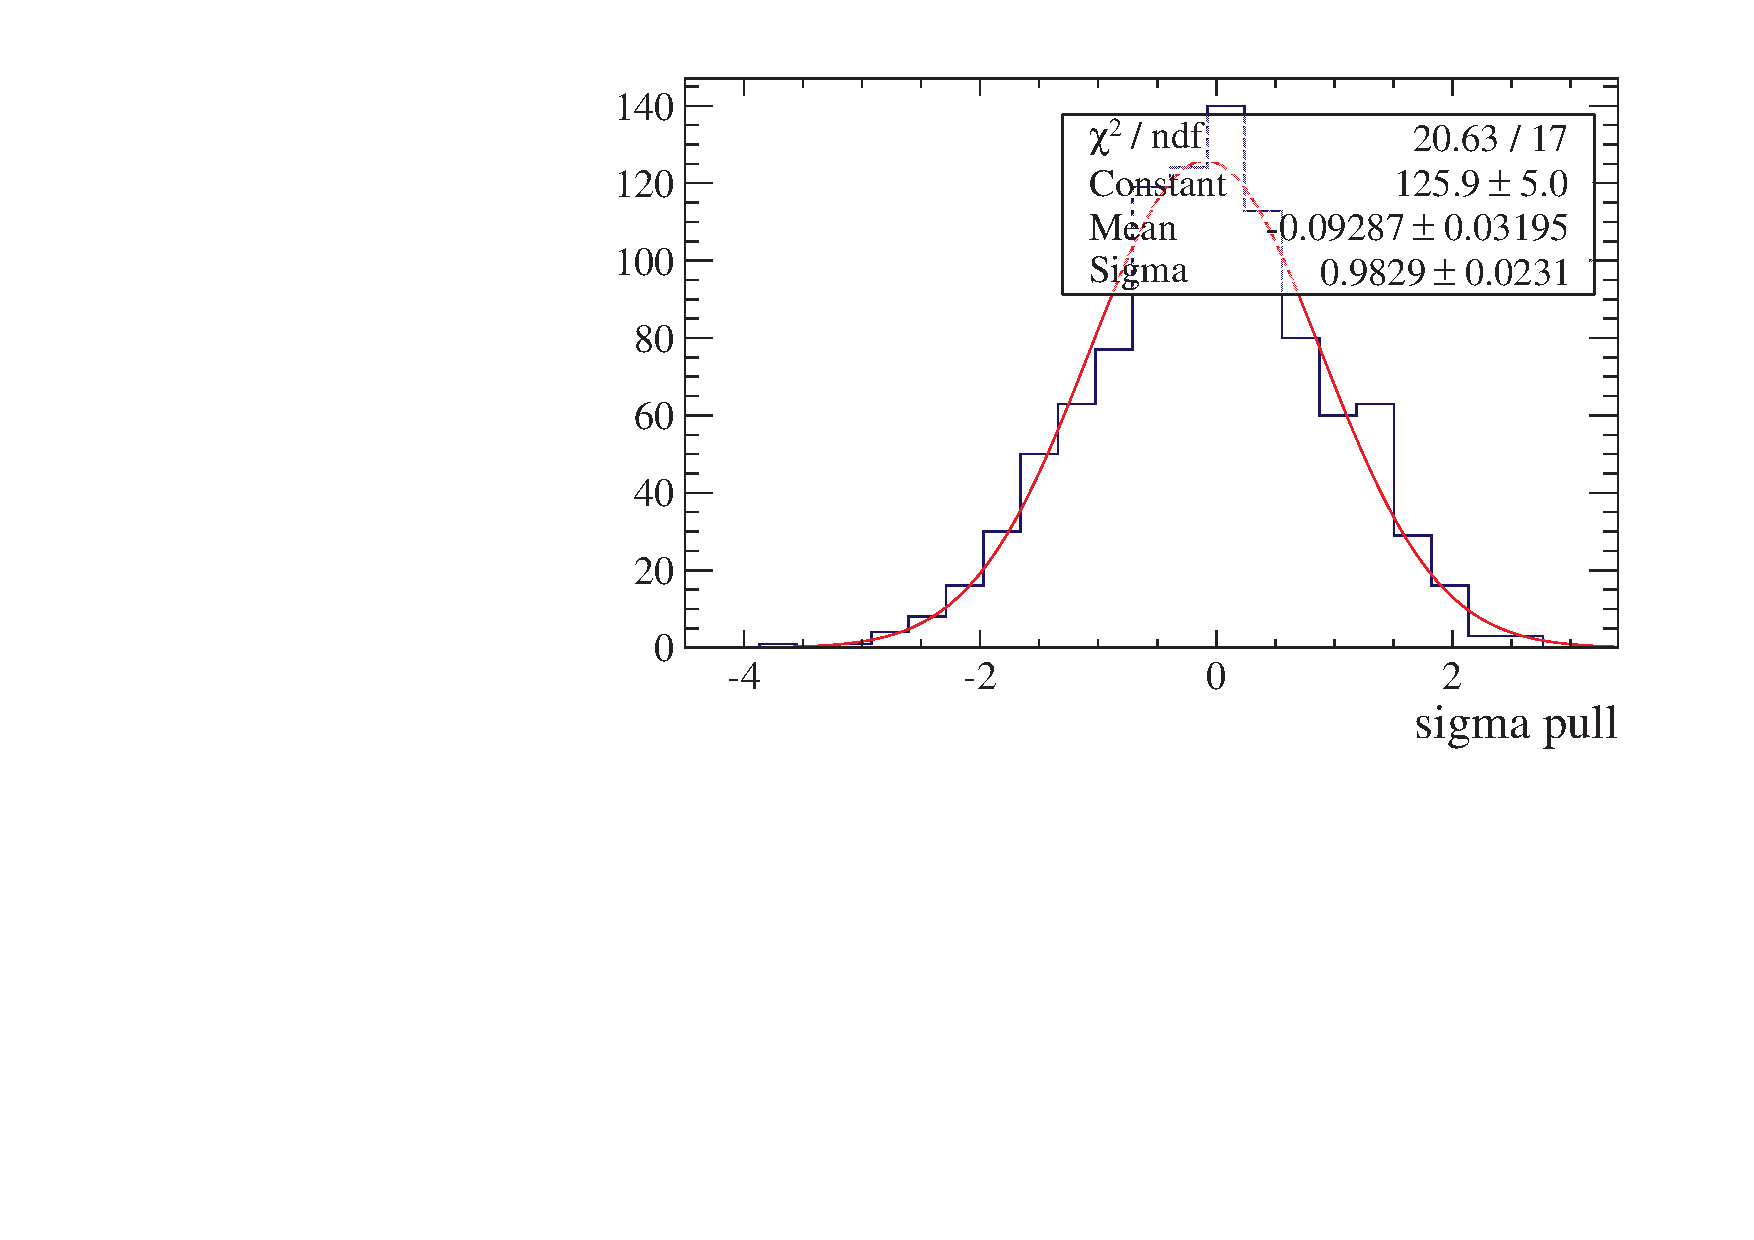
\includegraphics[width=0.5\textwidth]{./Output-1k/sigma_pull_c_thru.pdf}\end{center}
\end{frame}

\begin{frame}
\frametitle{My First Toy Study Output (10k studies) }\begin{center}
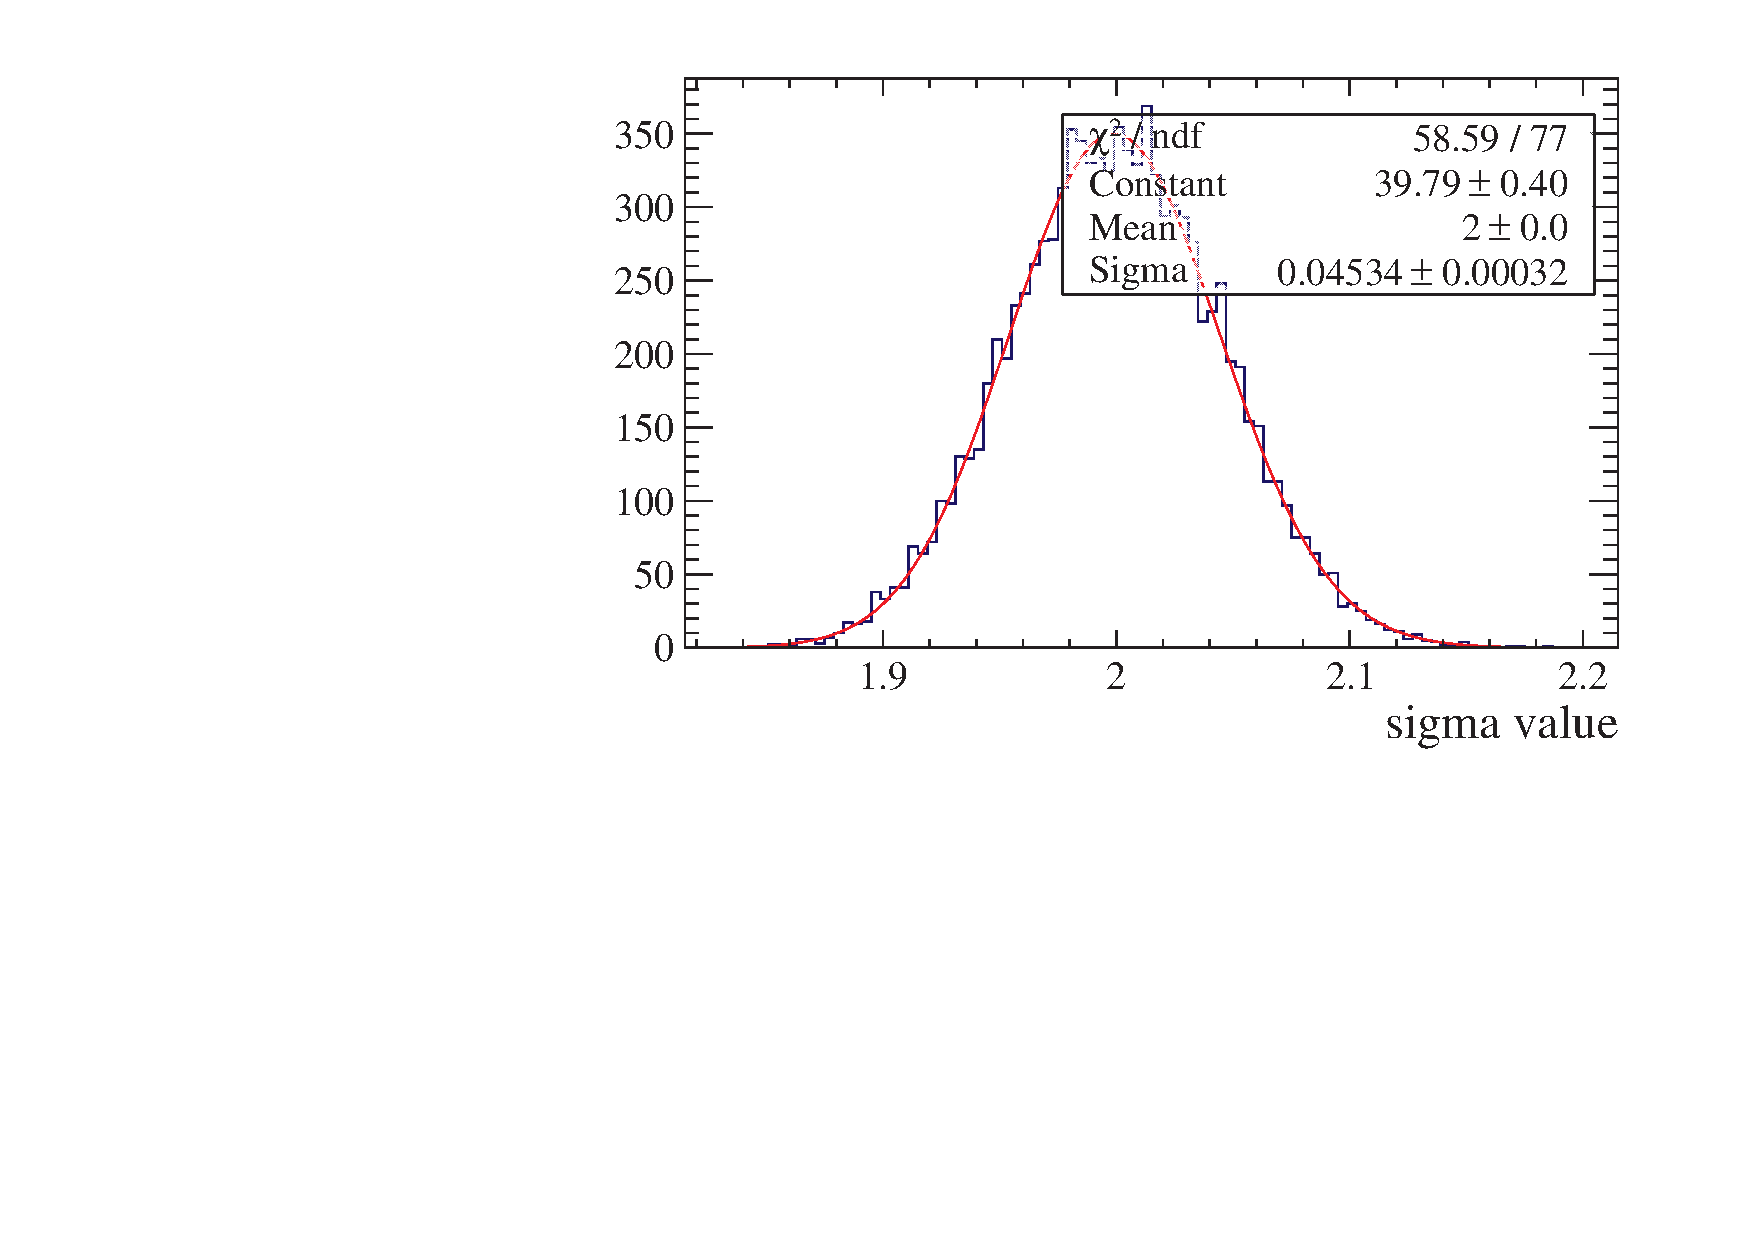
\includegraphics[width=0.5\textwidth]{./Output-10k/sigma_value_c_thru.pdf}
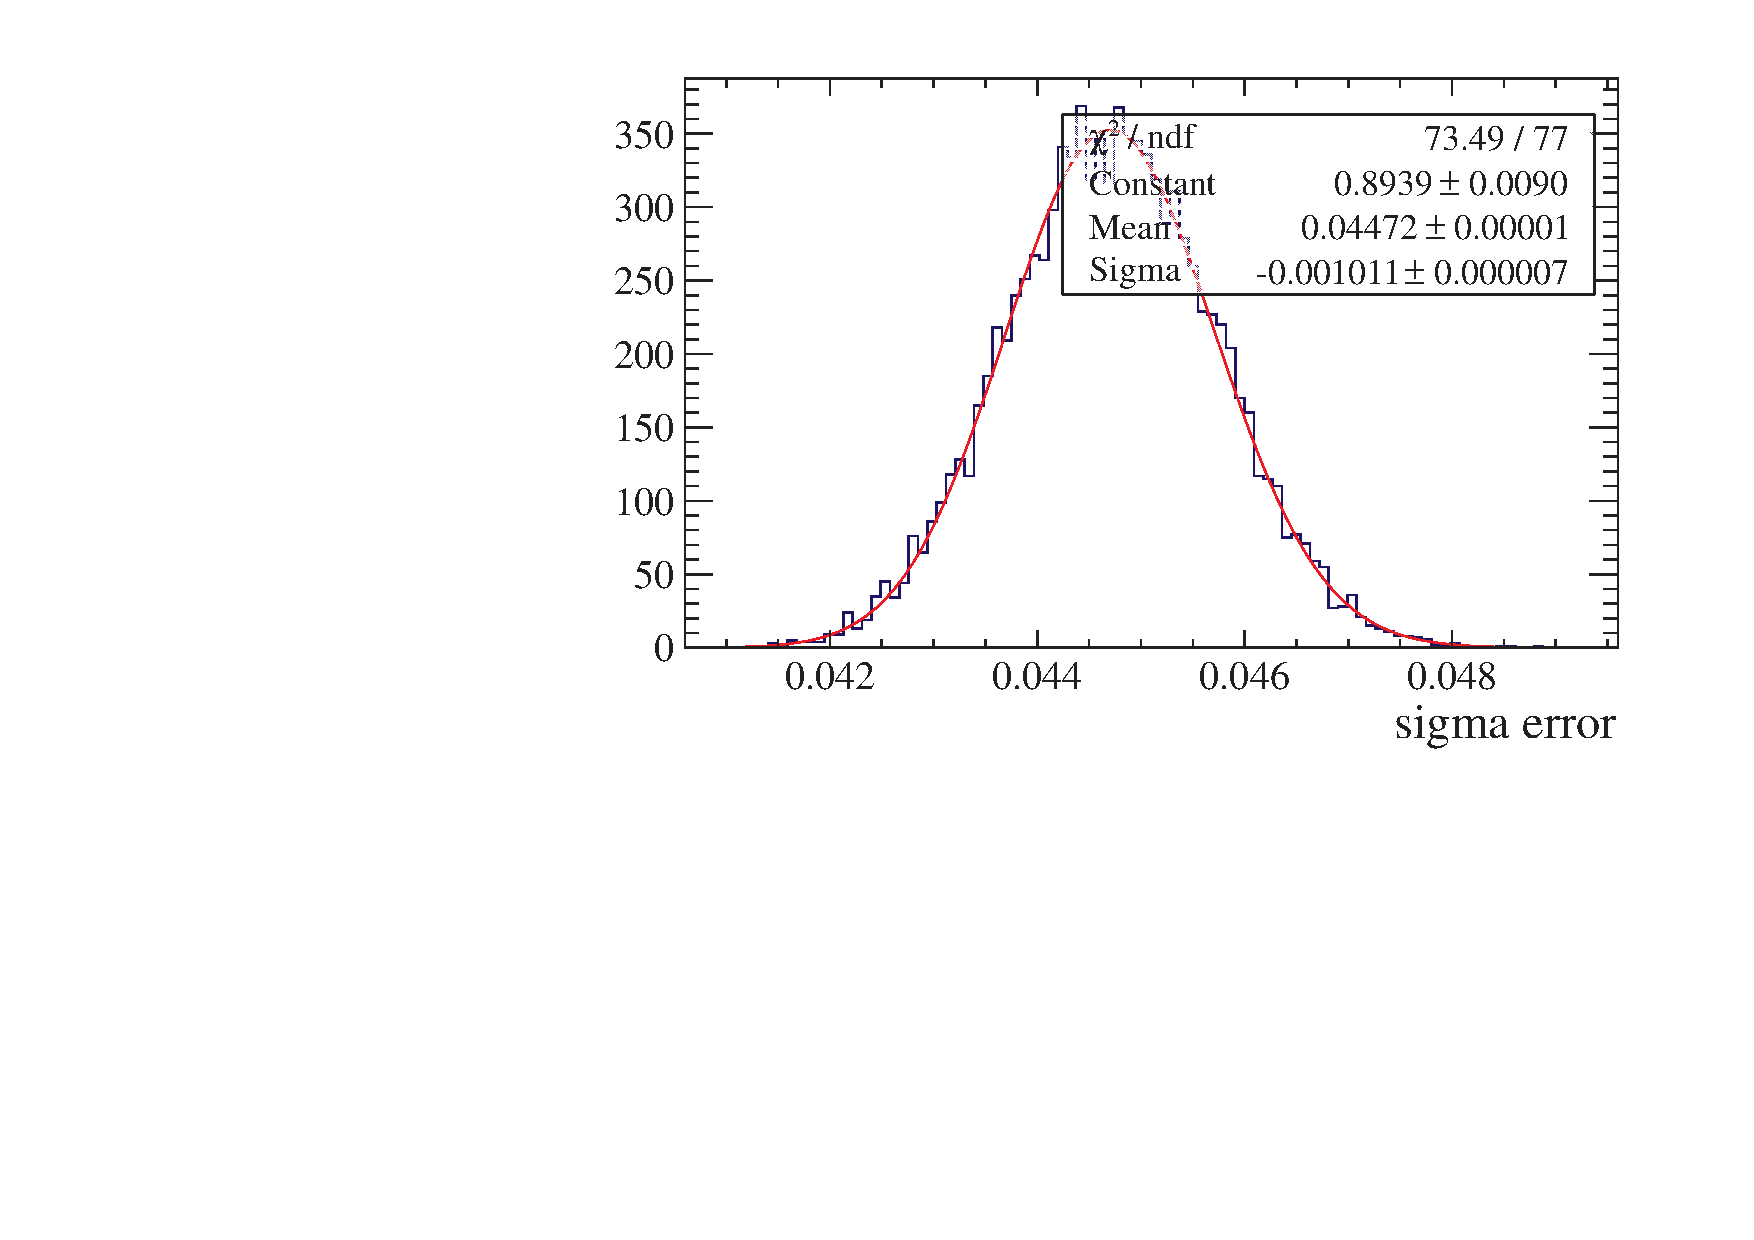
\includegraphics[width=0.5\textwidth]{./Output-10k/sigma_error_c_thru.pdf}\newline
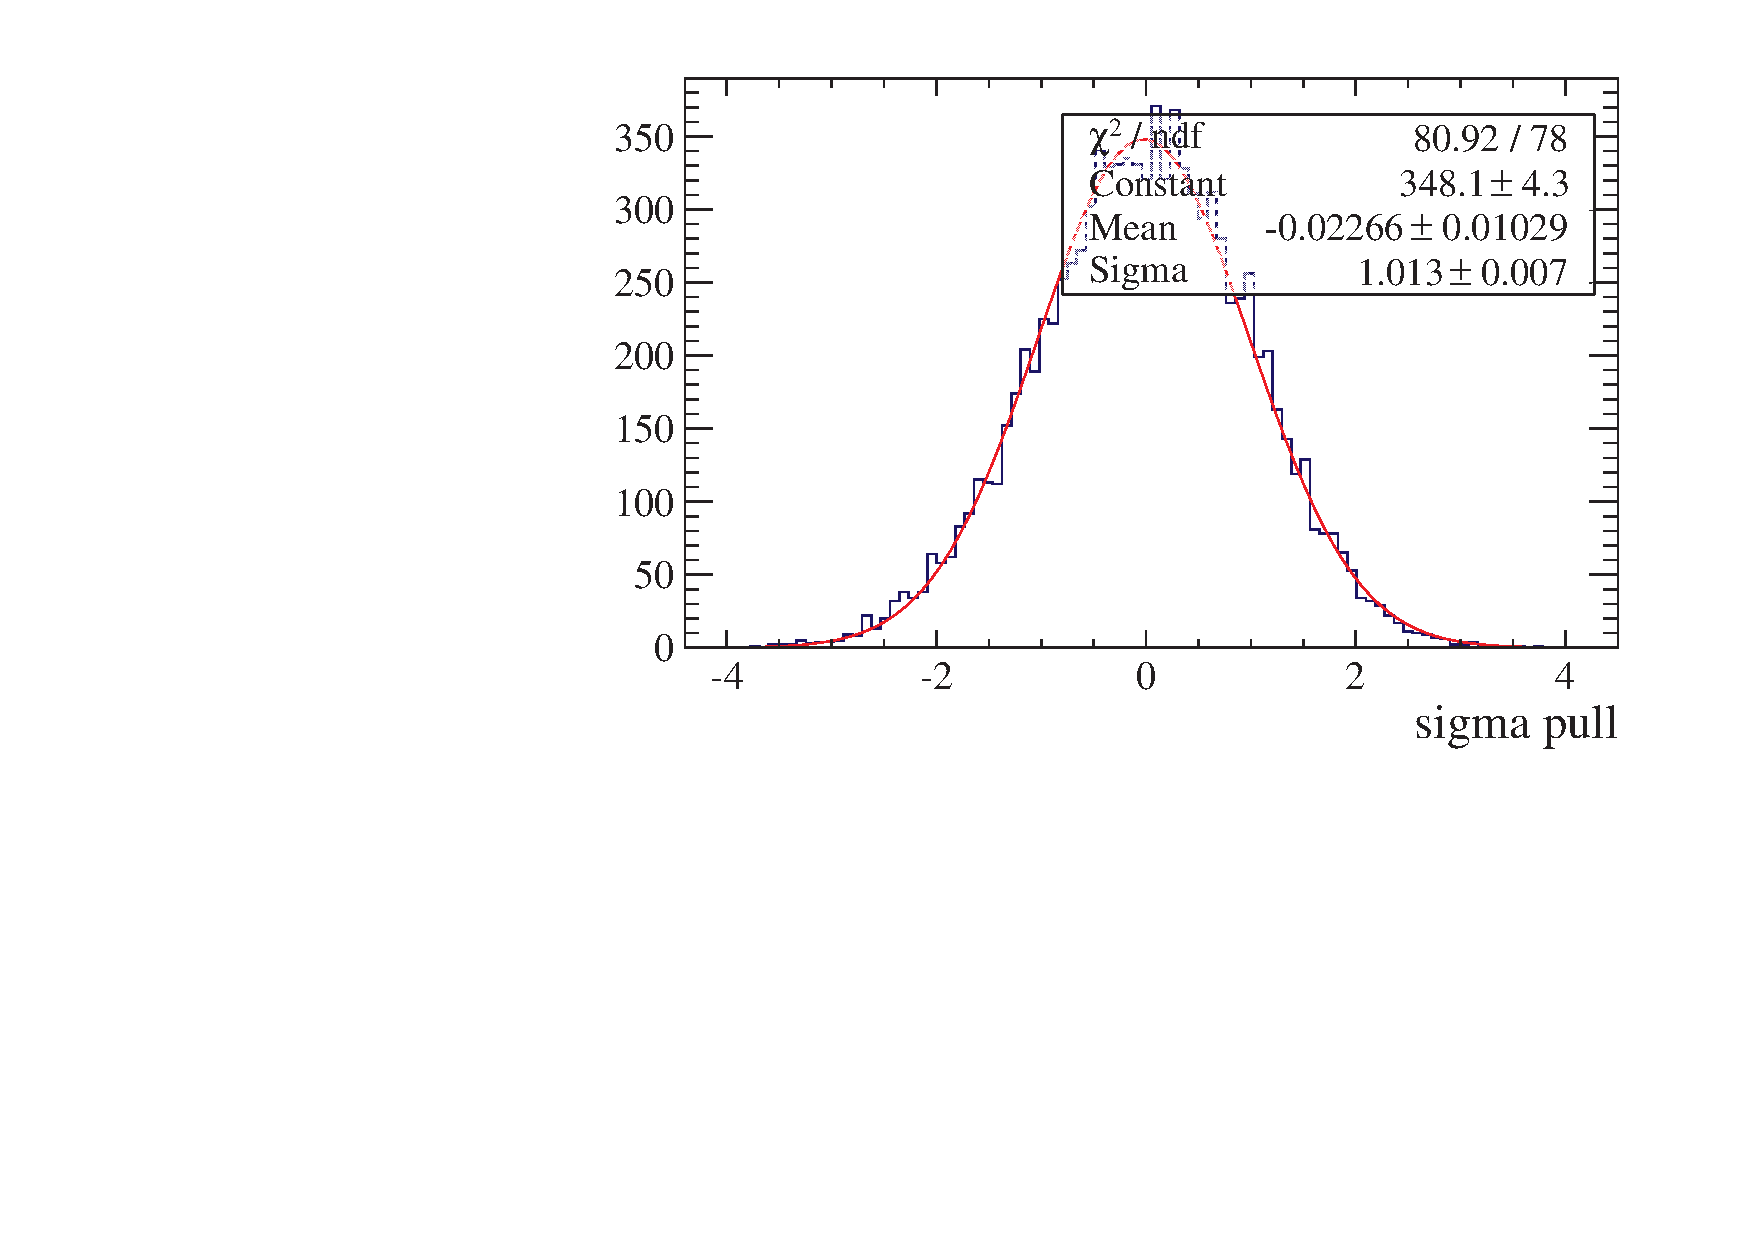
\includegraphics[width=0.5\textwidth]{./Output-10k/sigma_pull_c_thru.pdf}\end{center}
\end{frame}

\begin{frame}
\frametitle{My First Toy Study Output (100k studies) }\begin{center}
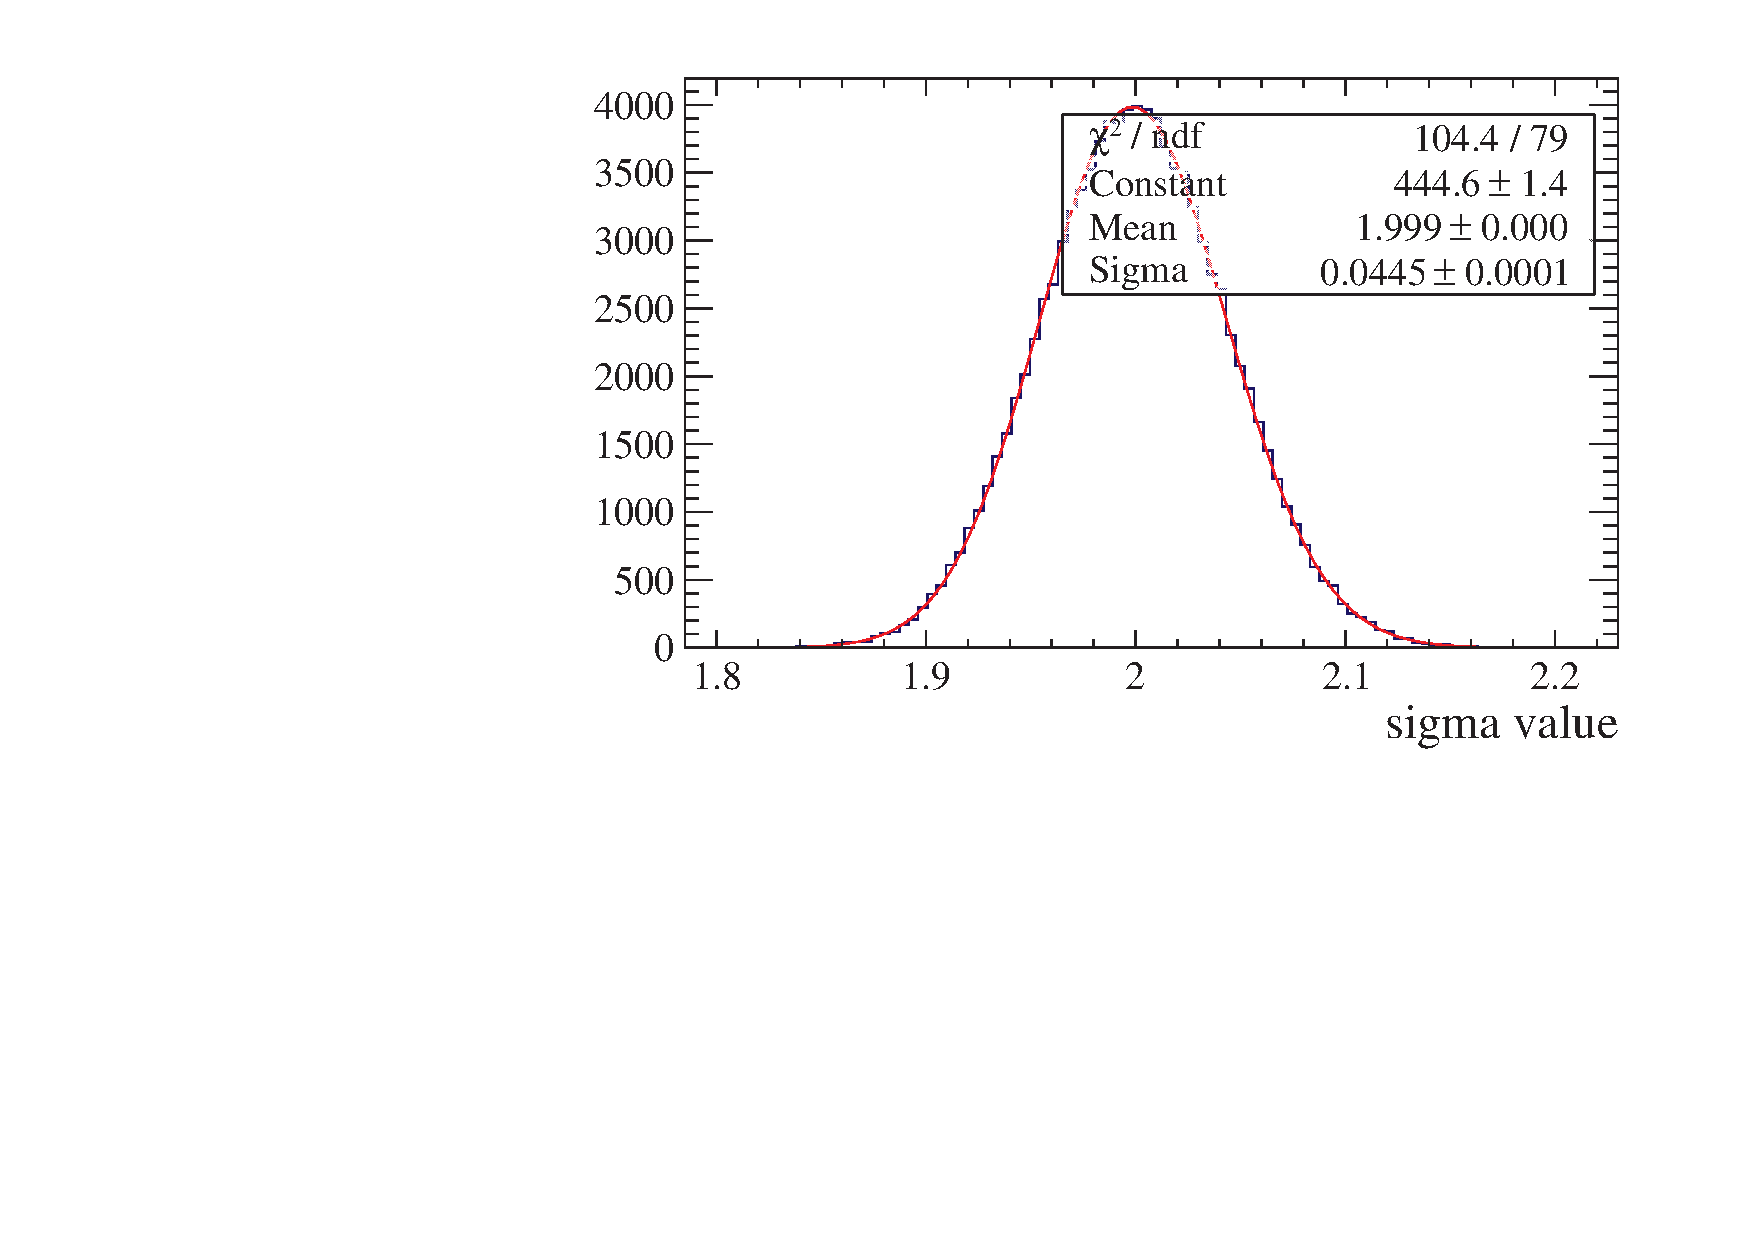
\includegraphics[width=0.5\textwidth]{./Output-100k/sigma_value_c_thru.pdf}
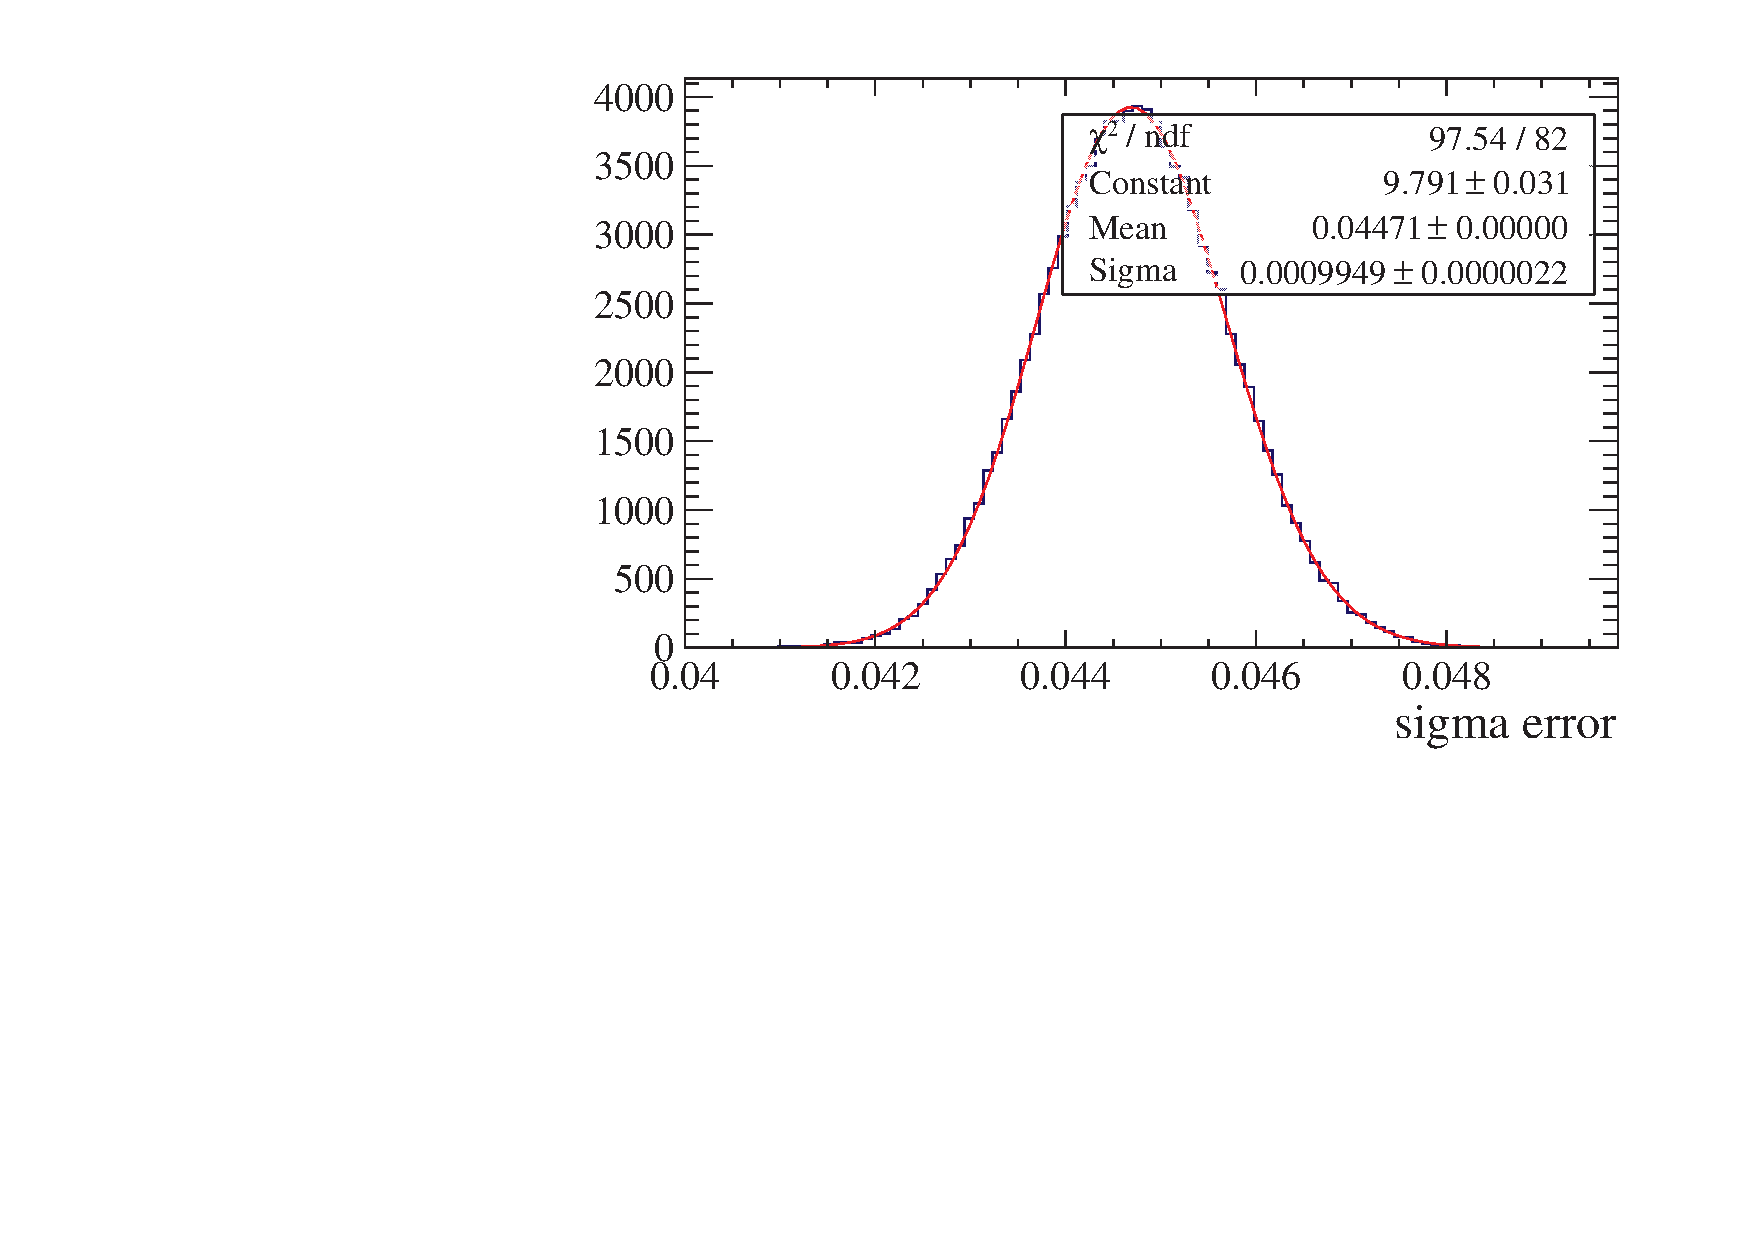
\includegraphics[width=0.5\textwidth]{./Output-100k/sigma_error_c_thru.pdf}\newline
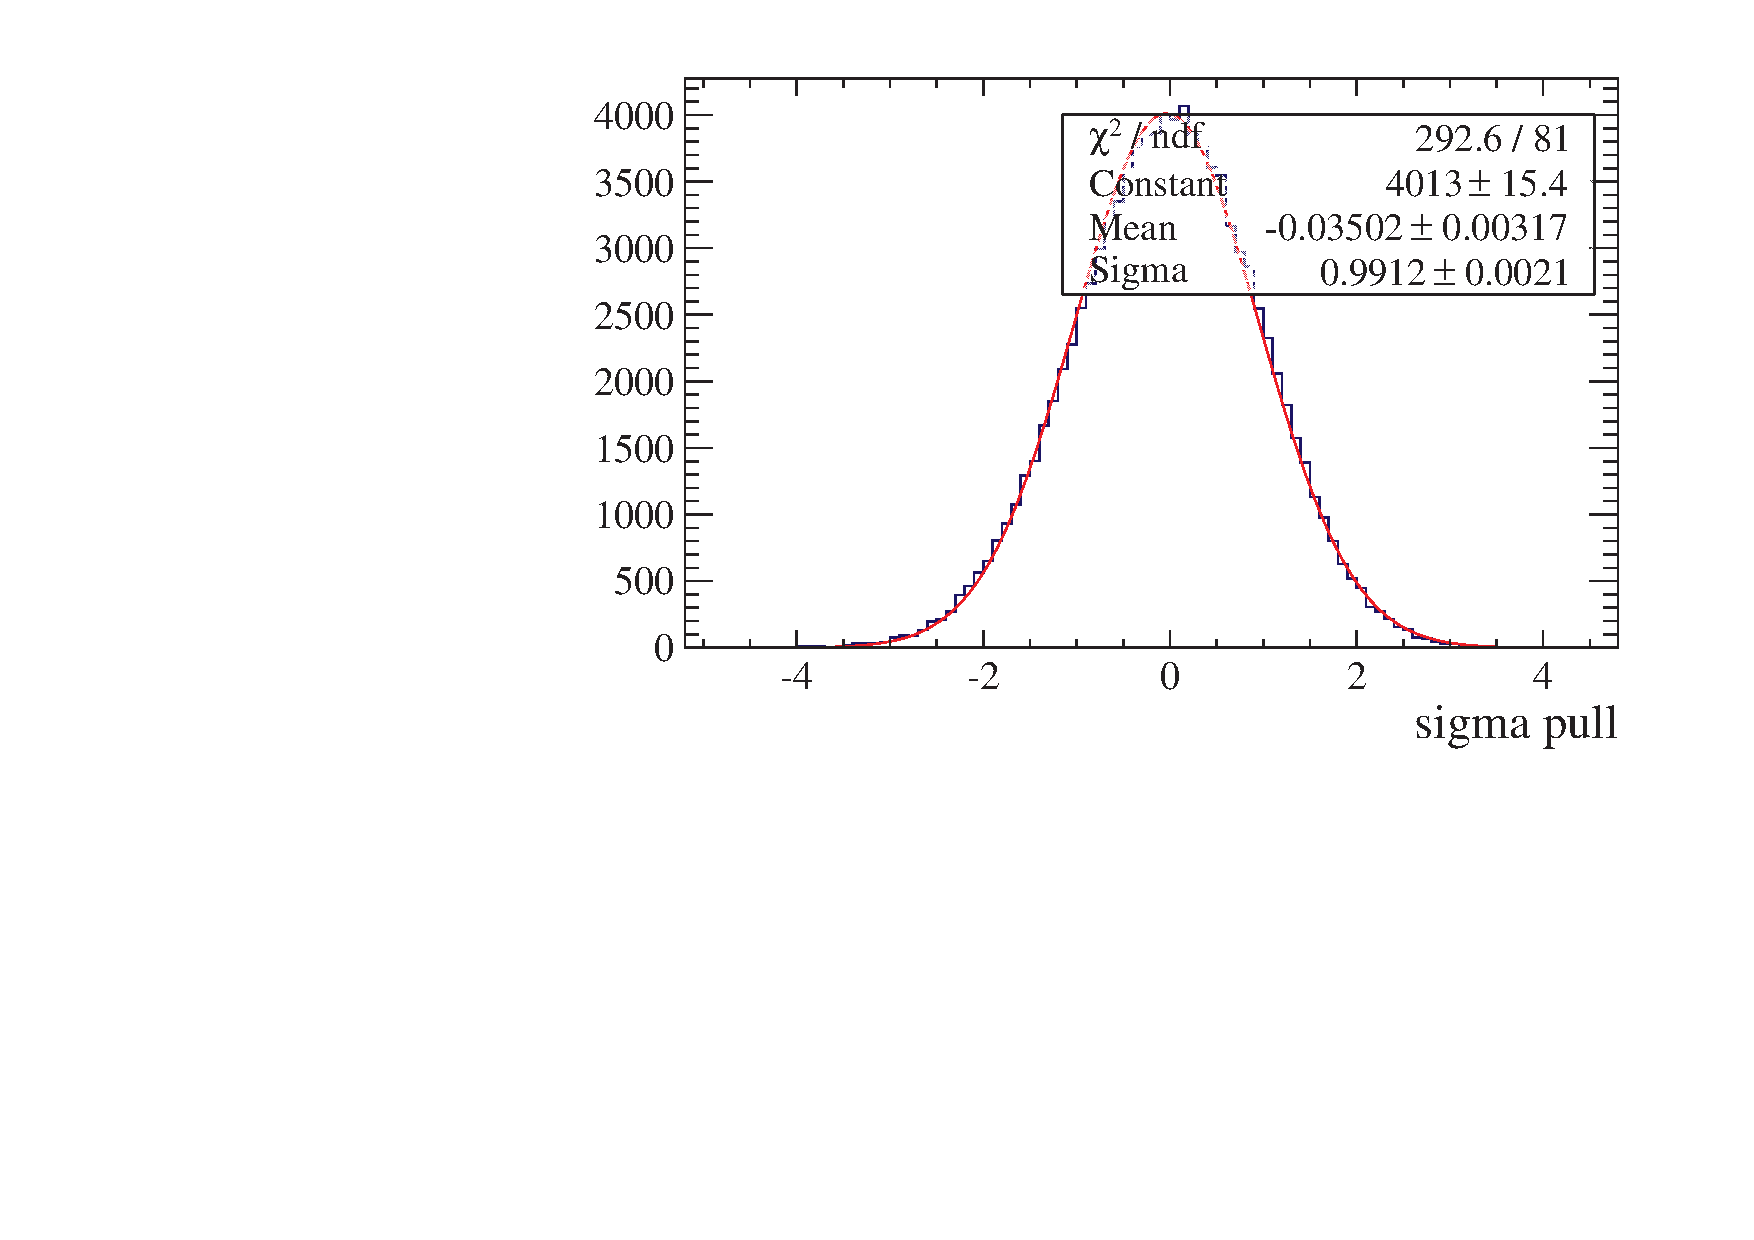
\includegraphics[width=0.5\textwidth]{./Output-100k/sigma_pull_c_thru.pdf}\end{center}
\end{frame}

\begin{frame}
\frametitle{Summary}
I've gone through the minimal required tools to run:\newline
\begin{itemize}
 \item Simple Foam fit
 \item $\Delta$LL scan
 \item Toy Study
 \item The most minimal PDF
 \item The most minimal XML\newline
\end{itemize}
A Minimal introduction to RapidFit.\newline

I will upload example PDFs and XML and email around where to find these in svn. I will be adding to this and can give a talk about once a week for the next month or so on useful RapidFit tools for everyone.
\end{frame}


\begin{frame}
\frametitle{RapidFit Utils}
I want to advertise the 'tools' in the utils directory.\newline\newline
Don't re-invent the wheel when it comes to working 'with' ROOT.\newline
I have many tools written to quickly/efficiently get information in/out of ROOT objects and into STL template objects.\newline

This includes many template functions.\newline

The code has been separated into source files building a small 'library' of common tasks which have been 'automated'.\newline
\end{frame}
\begin{frame}
\frametitle{Why care about things in the Utils Directory?}
There exist \textbf{many} pre-written functions to do things like:\newline\newline
Read in a branch of a TTree into a vector. \textbf{2 lines of code!}\newline
Read in a branch with a cut applied. \textbf{2 lines of code!}\newline
Names of TBranches in a TTree. \textbf{1 line of code!}\newline
Opening a TTree in a file regardless of name. \textbf{1 line of code!}\newline
List all Histograms in a file. \textbf{1 line of code!}\newline
Opening a File and checking it opened safely. \textbf{1 line of code!}\newline
Make a Histogram from a vector safely. \textbf{1 line of code!}\newline
Add a new TBranch to a TTree correctly. \textbf{1 line of code!}\newline

\end{frame}


\end{document}
